\begin{frame}{LR-KD: Learn from Rule-Corrected Targets}
    \small
    \textbf{Idea:} use rules during adaptation to create a teacher for a neural student.

    \vspace{0.75em}
    \centering
    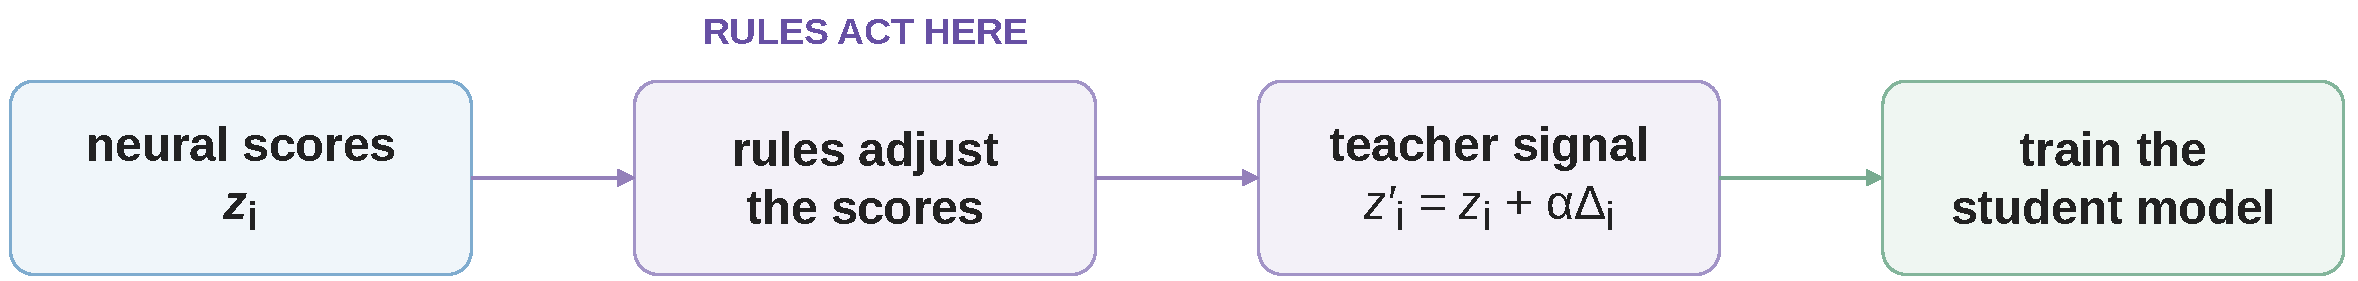
\includegraphics[width=0.94\linewidth]{figures/diagrams/lr_kd.pdf}

    \vspace{0.9em}
    \begin{columns}[T,onlytextwidth]
        \column{0.48\linewidth}
        \begin{beamercolorbox}[wd=\linewidth,sep=0.65em,rounded=true]{defbox}
            \textbf{Model change}\par
            \vspace{0.2em}
            The student learns from labels and rule-corrected model scores.
        \end{beamercolorbox}

        \column{0.48\linewidth}
        \begin{beamercolorbox}[wd=\linewidth,sep=0.65em,rounded=true]{takebox}
            \textbf{Deployment}\par
            \vspace{0.2em}
            Student model only; rules are no longer required.
        \end{beamercolorbox}
    \end{columns}
\end{frame}
